\documentclass[12pt,a4paper]{article}
\usepackage[T1]{fontenc}
\usepackage[utf8]{inputenc}
\usepackage[polish]{babel}
\usepackage{lmodern}
\usepackage{geometry}
\usepackage{setspace}
\usepackage{amsmath,amssymb}
\usepackage{graphicx}
\usepackage{float}
\usepackage{booktabs}
\usepackage{caption}
\usepackage{listings}
\usepackage{xcolor}
\usepackage{hyperref}

\geometry{margin=2.5cm}
\onehalfspacing
\captionsetup{font=small,labelfont=bf}

\lstdefinestyle{pythonstyle}{
    language=Python,
    basicstyle=\ttfamily\small,
    keywordstyle=\color{blue},
    commentstyle=\color{teal},
    stringstyle=\color{purple},
    showstringspaces=false,
    frame=single,
    breaklines=true
}

\begin{document}

\begin{titlepage}
    \centering
    {\large Politechnika / Uczelnia \par}
    \vspace{1.5cm}
    {\Large\bfseries Wieloetapowe procesy decyzyjne, Laboratorium 04\par}
    \vspace{1.2cm}
    {\large Przedmiot: Wprowadzenie do Przetwarzania Danych / WPD\par}
    \vspace{2cm}
    \begin{flushleft}
        \textbf{Autor:} Stanis\l{}aw Krupa \\
        \textbf{Nr albumu:} 254977 \\
        \textbf{Grupa:} XX \\
        \textbf{Prowadz\k{a}cy:} dr in\.z. Marlena Dr\k{a}g \\
        \textbf{Data wykonania:} 20.04.2026 \\
    \end{flushleft}
    \vfill
    {\large \today \par}
\end{titlepage}

\section{Cel pracy}
Celem laboratorium by\l{}o praktyczne poznanie metod analizy uk\l{}ad\'ow dynamicznych w kontek\'scie chaosu oraz stabilno\'sci. W ramach \'{c}wiczenia nale\.za\l{}o oszacowa\'c stopie\'n chaotyczno\'sci uk\l{}adu deterministycznego z wykorzystaniem wyk\l{}adnika Lapunowa, zdefiniowa\'c stabilno\'s\'c w sensie Lapunowa oraz sprawdzi\'c stabilno\'s\'c wybranego uk\l{}adu dwiema klasycznymi metodami Lapunowa.

\section{Opis zada\'n realizowanych na zaj\k{e}ciach}
Podczas zaj\k{e}\'c analizowano trzy zagadnienia zwi\k{a}zane z teori\k{a} uk\l{}ad\'ow dynamicznych:
\begin{itemize}
    \item \textbf{Ocena chaosu w uk\l{}adzie deterministycznym} -- badano, jak szybko rozchodz\k{a} si\k{e} dwie pocz\k{a}tkowo bliskie trajektorie w czasie i jak na tej podstawie wyznaczy\'c maksymalny wyk\l{}adnik Lapunowa.
    \item \textbf{Poj\k{e}cie stabilno\'sci} -- uporz\k{a}dkowano definicje stabilno\'sci rozwi\k{a}za\'n, ze szczeg\'olnym naciskiem na stabilno\'s\'c w sensie Lapunowa i stabilno\'s\'c asymptotyczn\k{a}.
    \item \textbf{Badanie stabilno\'sci metodami Lapunowa} -- dla wybranego uk\l{}adu nieliniowego wykonano linearyzacj\k{e} (metoda pierwsza) oraz om\'owiono kryterium funkcji Lapunowa (metoda druga).
\end{itemize}

\section{Podstawy teoretyczne}

\subsection{Wyk\l{}adnik Lapunowa a chaos}
Dla dw\'och trajektorii oddalonych pocz\k{a}tkowo o $d_0$:
\begin{equation}
    d(t) \approx d_0 e^{\lambda t},
\end{equation}
gdzie $\lambda$ to wyk\l{}adnik Lapunowa. Po przekszta\l{}ceniu:
\begin{equation}
    \ln\left(\frac{d(t)}{d_0}\right) \approx \lambda t.
\end{equation}
Je\'sli $\lambda_{\max} > 0$, uk\l{}ad wykazuje chaos (wra\.zliwo\'s\'c na warunki pocz\k{a}tkowe).

\subsection{Definicja stabilno\'sci w sensie Lapunowa}
Niech $x^\ast$ b\k{e}dzie punktem r\'ownowagi uk\l{}adu $\dot{x}=f(x)$.
Punkt $x^\ast$ jest \textbf{stabilny w sensie Lapunowa}, je\'sli:
\begin{equation}
    \forall \varepsilon > 0 \ \exists \delta > 0:
    \|x(0)-x^\ast\| < \delta \Rightarrow \|x(t)-x^\ast\| < \varepsilon \ \text{dla ka\.zdego } t \ge 0.
\end{equation}
Je\.zeli dodatkowo:
\begin{equation}
    \lim_{t\to\infty}x(t)=x^\ast,
\end{equation}
to punkt r\'ownowagi jest stabilny asymptotycznie.

\subsection{Pierwsza i druga metoda Lapunowa}
\textbf{Pierwsza metoda Lapunowa} polega na linearyzacji uk\l{}adu w otoczeniu punktu r\'ownowagi i analizie warto\'sci w\l{}asnych macierzy Jacobiego.\\
\textbf{Druga metoda Lapunowa} opiera si\k{e} na znalezieniu funkcji $V(x)$ spe\l{}niaj\k{a}cej warunki dodatniej okre\'slono\'sci oraz ujemnej (p\'o\l{}-)okre\'slono\'sci pochodnej wzd\l{}u\.z trajektorii:
\begin{equation}
    \dot{V}(x)=\nabla V(x)\cdot f(x).
\end{equation}

\section{Spos\'ob rozwi\k{a}zania zada\'n i komentarz}

\subsection{Zadanie 1 -- oszacowanie stopnia chaosu (uk\l{}ad Lorenza)}
W notatniku zasymulowano klasyczny uk\l{}ad Lorenza:
\begin{equation}
    \begin{cases}
        \dot{x}=\sigma(y-x), \\
        \dot{y}=x(r-z)-y, \\
        \dot{z}=xy-bz,
    \end{cases}
\end{equation}
dla parametr\'ow $\sigma=10$, $r=28$, $b=\frac{8}{3}$. Nast\k{e}pnie uruchomiono dwie symulacje, kt\'orych warunki pocz\k{a}tkowe r\'o\.zni\l{}y si\k{e} perturbacj\k{a} $d_0=10^{-8}$. Obliczono:
\begin{equation}
    d(t)=\sqrt{(x_2-x_1)^2+(y_2-y_1)^2+(z_2-z_1)^2},
\end{equation}
oraz przebieg $\ln(d(t)/d_0)$.

W celu estymacji $\lambda_{\max}$ wybrano zakres czasowy, w kt\'orym zale\.zno\'s\'c logarytmicznej dywergencji od czasu jest w przybli\.zeniu liniowa (\emph{Expansion Range}: indeksy $k_{\min}=1000$, $k_{\max}=2500$), a nast\k{e}pnie wykonano regresj\k{e} liniow\k{a}. Otrzymane dodatnie nachylenie prostej oznacza dodatni wyk\l{}adnik Lapunowa, czyli chaotyczny charakter dynamiki.\\
\textbf{Komentarz:} najwa\.zniejszym elementem tej metody jest poprawny dob\'or zakresu dopasowania; zbyt kr\'otki lub zbyt p\'o\'zny zakres (po nasyceniu) mo\.ze zniekszta\l{}ci\'c estymacj\k{e}.

\begin{figure}[H]
    \centering
    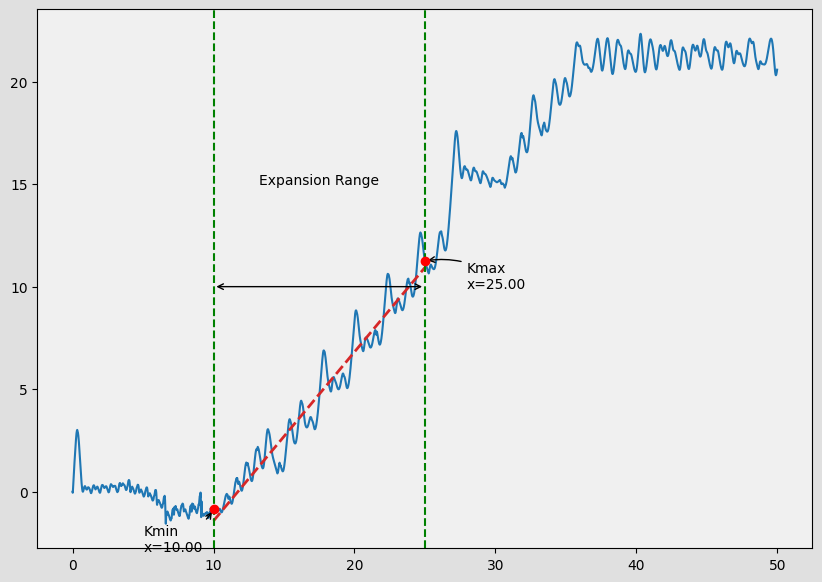
\includegraphics[width=0.9\linewidth]{zadanie1.png}
    \caption{Estymacja maksymalnego wyk\l{}adnika Lapunowa na podstawie dywergencji trajektorii uk\l{}adu Lorenza.}
    \label{fig:lyapunov}
\end{figure}

\subsection{Zadanie 2 -- stabilno\'s\'c uk\l{}adu w sensie Lapunowa}
Dla uk\l{}adu
\begin{equation}
    \begin{cases}
        \dot{x}_1=x_1^2-2x_1, \\
        \dot{x}_2=\frac{1}{x_2}-x_1+1,
    \end{cases}
\end{equation}
zrealizowano analiz\k{e} zgodnie z procedur\k{a} podan\k{a} na zaj\k{e}ciach.

\paragraph{Krok 1. Wyznaczenie punkt\'ow r\'ownowagi.}
Rozwi\k{a}zano uk\l{}ad r\'owna\'n $\dot{x}_1=0$, $\dot{x}_2=0$:
\begin{equation}
    x_1^2-2x_1=0,\qquad \frac{1}{x_2}-x_1+1=0.
\end{equation}
Otrzymano dwa punkty r\'ownowagi:
\begin{equation}
    P_1=(0,-1),\qquad P_2=(2,1).
\end{equation}

\paragraph{Krok 2. Linearyzacja (szereg Taylora wok\'o\l{} punktu r\'ownowagi).}
W otoczeniu punktu r\'ownowagi $P$ przyjmujemy:
\begin{equation}
    \dot{\xi} \approx J(P)\,\xi,
\end{equation}
gdzie $\xi=x-P$ jest ma\l{}ym odchyleniem, a $J(P)$ to Jacobian policzony w punkcie r\'ownowagi.
W laboratorium skupiono si\k{e} przede wszystkim na wyznaczeniu Jacobianu i jego warto\'sci w punktach r\'ownowagi.

\paragraph{Krok 3. Obliczenie Jacobianu.}
Dla $f_1(x_1,x_2)=x_1^2-2x_1$ oraz $f_2(x_1,x_2)=\frac{1}{x_2}-x_1+1$:
\begin{equation}
    J(x_1,x_2)=
    \begin{bmatrix}
        \frac{\partial f_1}{\partial x_1} & \frac{\partial f_1}{\partial x_2}\\
        \frac{\partial f_2}{\partial x_1} & \frac{\partial f_2}{\partial x_2}
    \end{bmatrix}
    =
    \begin{bmatrix}
        2x_1-2 & 0\\
        -1 & -\frac{1}{x_2^2}
    \end{bmatrix}.
\end{equation}

\paragraph{Krok 4. Warto\'sci Jacobianu w punktach r\'ownowagi.}
\begin{equation}
    J(P_1)=J(0,-1)=
    \begin{bmatrix}
        -2 & 0\\
        -1 & -1
    \end{bmatrix},
    \qquad
    J(P_2)=J(2,1)=
    \begin{bmatrix}
        2 & 0\\
        -1 & -1
    \end{bmatrix}.
\end{equation}

\paragraph{Krok 5. Badanie stabilno\'sci przez warto\'sci w\l{}asne Jacobianu.}
\begin{equation}
    \lambda\big(J(P_1)\big)=\{-2,-1\},\qquad
    \lambda\big(J(P_2)\big)=\{2,-1\}.
\end{equation}
Interpretacja:
\begin{itemize}
    \item dla $P_1=(0,-1)$ wszystkie cz\k{e}\'sci rzeczywiste warto\'sci w\l{}asnych s\k{a} ujemne, wi\k{e}c punkt jest lokalnie asymptotycznie stabilny;
    \item dla $P_2=(2,1)$ jedna warto\'s\'c w\l{}asna jest dodatnia, wi\k{e}c punkt jest niestabilny (typ siod\l{}owy).
\end{itemize}

\textbf{Komentarz:} stabilno\'s\'c w sensie Lapunowa w praktyce sprawdzono przez linearyzacj\k{e} i spektrum Jacobianu. Wyniki dla obu punkt\'ow s\k{a} rozr\'o\.znialne i jednoznaczne: $P_1$ stabilny lokalnie, $P_2$ niestabilny.

\subsection{Zadanie 3 -- badanie stabilno\'sci dwiema metodami Lapunowa}
W trzeciej kom\'orce notatnika przeanalizowano uk\l{}ad skalarowy:
\begin{equation}
    \dot{x}=-x.
\end{equation}
Punkt r\'ownowagi wynika z warunku $\dot{x}=0$, zatem:
\begin{equation}
    x^\ast=0.
\end{equation}

\paragraph{Pierwsza metoda Lapunowa (linearyzacja).}
Dla uk\l{}adu skalarowego Jacobian jest pochodn\k{a} prawej strony:
\begin{equation}
    J(x)=\frac{d(-x)}{dx}=-1.
\end{equation}
W punkcie r\'ownowagi $x^\ast=0$ otrzymujemy warto\'s\'c w\l{}asn\k{a} $\lambda=-1<0$, co oznacza lokaln\k{a} asymptotyczn\k{a} stabilno\'s\'c punktu r\'ownowagi.

\paragraph{Druga metoda Lapunowa (funkcja Lapunowa).}
Przyj\k{e}to funkcj\k{e}:
\begin{equation}
    V(x)=x^2.
\end{equation}
Jej pochodna po czasie wzd\l{}u\.z trajektorii uk\l{}adu:
\begin{equation}
    \dot{V}(x)=\frac{dV}{dx}\dot{x}=2x\cdot(-x)=-2x^2.
\end{equation}
Sprawdzenie warunk\'ow z zaj\k{e}\'c:
\begin{equation}
    V(x)>0\ \text{dla}\ x\neq 0,\qquad \dot{V}(x)<0\ \text{dla}\ x\neq 0,
\end{equation}
\begin{equation}
    V(0)=0,\qquad \dot{V}(0)=0.
\end{equation}
Warunki s\k{a} spe\l{}nione, wi\k{e}c punkt r\'ownowagi $x^\ast=0$ jest asymptotycznie stabilny.

\textbf{Komentarz:} w tym zadaniu obie metody Lapunowa s\k{a} zgodne i prowadz\k{a} do tego samego wniosku o stabilno\'sci asymptotycznej. Druga metoda dodatkowo daje bezpo\'sredni dow\'od poprzez znak funkcji $V$ i jej pochodnej.

\section{Wnioski}
Przeprowadzona analiza potwierdzi\l{}a, \.ze wyk\l{}adniki Lapunowa s\k{a} skutecznym narz\k{e}dziem do ilo\'sciowej oceny chaosu w uk\l{}adach deterministycznych. Dodatni maksymalny wyk\l{}adnik Lapunowa dla uk\l{}adu Lorenza wskazuje na siln\k{a} wra\.zliwo\'s\'c na warunki pocz\k{a}tkowe. Dla analizowanego uk\l{}adu nieliniowego punkt $(2,1)$ okaza\l{} si\k{e} niestabilny, co wynika bezpo\'srednio z analizy warto\'sci w\l{}asnych Jacobiego. Otrzymane rezultaty pokazuj\k{a} zgodno\'s\'c podej\'scia numerycznego i analitycznego przy badaniu stabilno\'sci.

\section{Bibliografia}
\begin{enumerate}
    \item H. K. Khalil, \textit{Nonlinear Systems}, Prentice Hall, 3rd ed., 2002.
    \item S. H. Strogatz, \textit{Nonlinear Dynamics and Chaos}, Westview Press, 2nd ed., 2015.
    \item E. Ott, \textit{Chaos in Dynamical Systems}, Cambridge University Press, 2nd ed., 2002.
    \item Dokumentacja bibliotek: NumPy, SciPy, SymPy, Matplotlib, \url{https://docs.scipy.org/}, \url{https://docs.sympy.org/}.
\end{enumerate}

\section{Za\l{}\k{a}czniki}
\subsection*{Za\l{}\k{a}cznik A -- kod do estymacji wyk\l{}adnika Lapunowa}
\begin{lstlisting}[style=pythonstyle]
import numpy as np
from scipy.integrate import solve_ivp

sigma, r, b = 10.0, 28.0, 8/3.0
def lorenz(t, state):
    x, y, z = state
    return [sigma*(y-x), x*(r-z)-y, x*y-b*z]

dist_0 = 1e-8
# ... dwie bliskie trajektorie, dystans, logarytm i dopasowanie liniowe ...
\end{lstlisting}

\subsection*{Za\l{}\k{a}cznik B -- kod do analizy stabilno\'sci (Jacobiego)}
\begin{lstlisting}[style=pythonstyle]
import sympy as sp
x1, x2 = sp.symbols('x1 x2')
f1 = x1**2 - 2*x1
f2 = 1/x2 - x1 + 1
J = sp.Matrix([f1, f2]).jacobian([x1, x2])
J_at_P = J.subs({x1: 2, x2: 1})
print(J_at_P.eigenvals())  # [2, -1]
\end{lstlisting}

\end{document}
